\section{Transformer-Based LTSF Solutions}
\label{sec:trans}


\begin{figure*}[t]
\vspace{-0.2cm}
\begin{center}
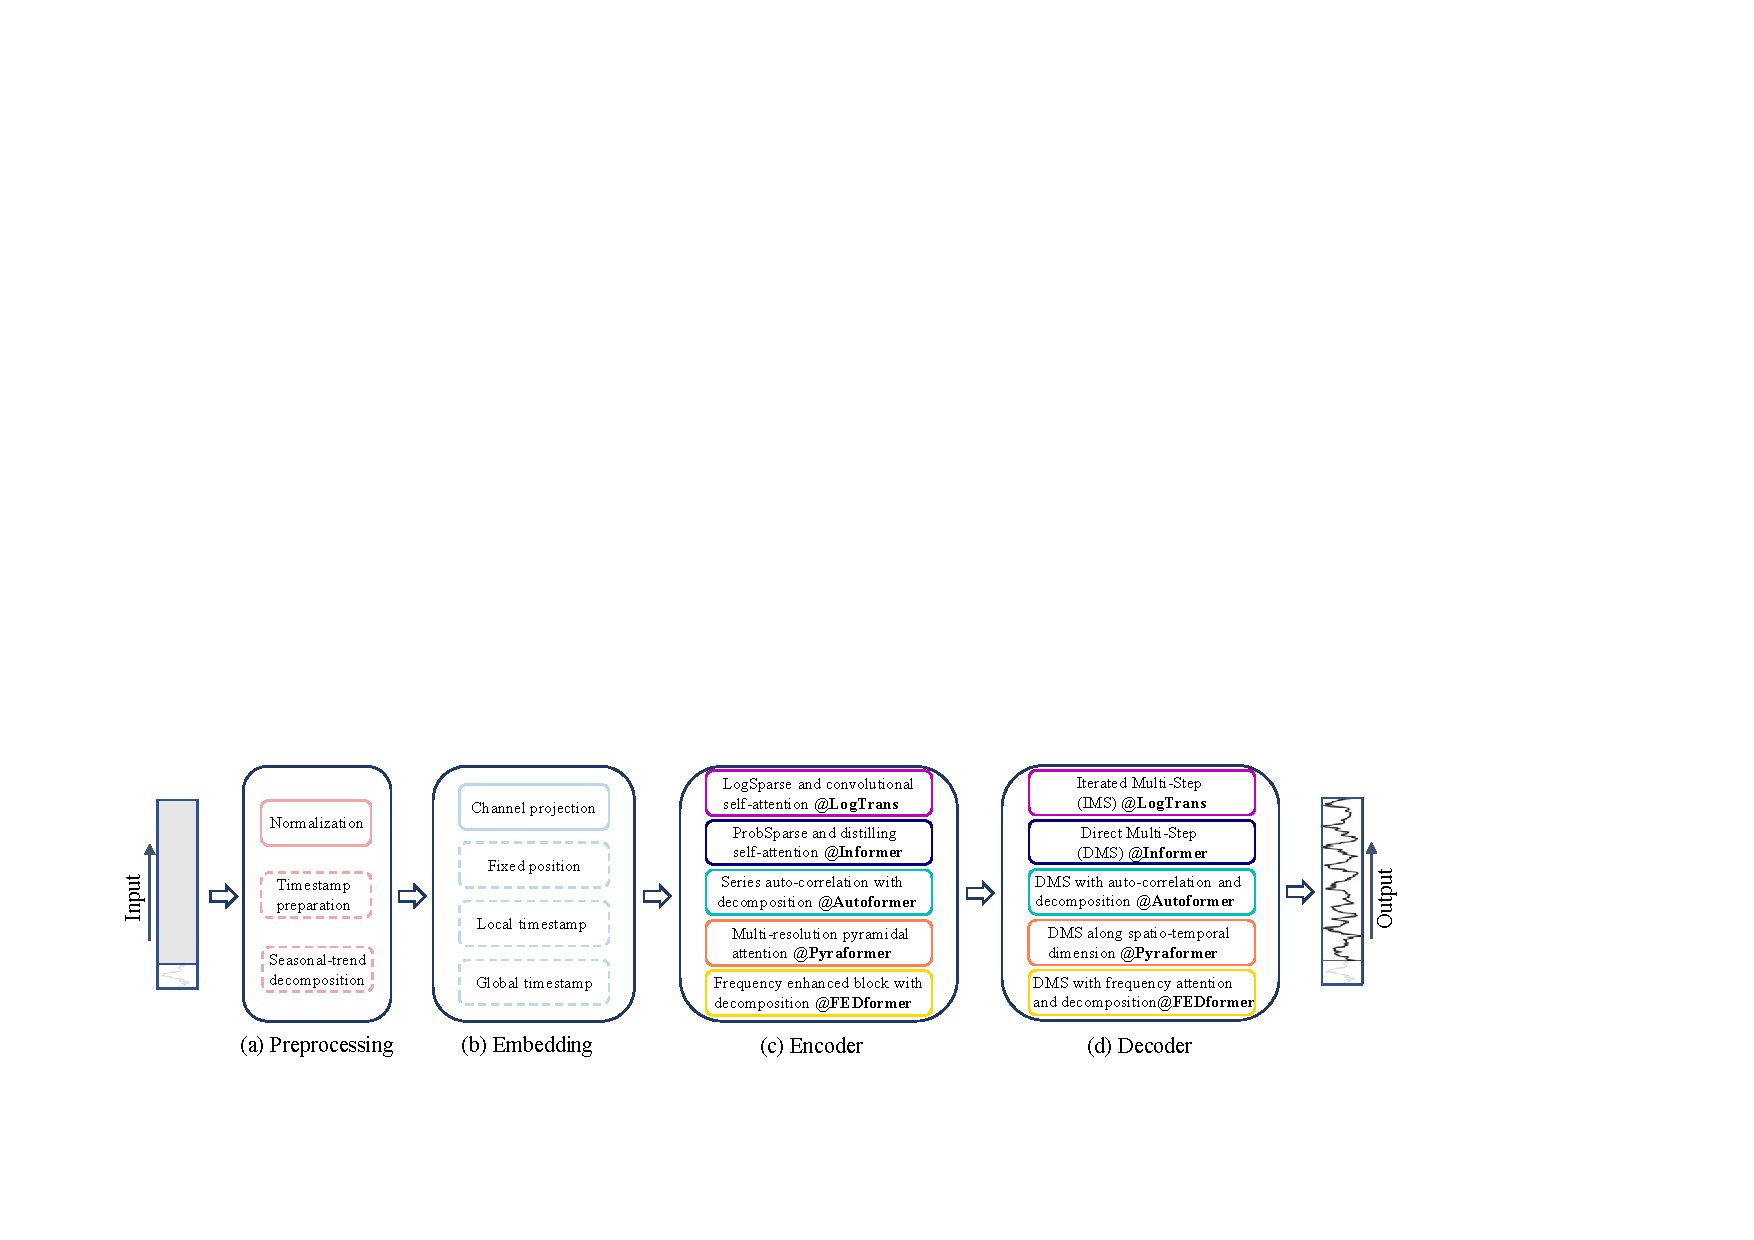
\includegraphics[width=1\textwidth]{img/pipeline.pdf}
\end{center}
\vspace{-0.4cm}
\caption{The pipeline of existing Transformer-based TSF solutions. In (a) and (b), the solid boxes are essential operations, and the dotted boxes are applied optionally. (c) and (d) are distinct for different methods~\cite{li2019LogTrans,informer,xu2021autoformer,liu2021pyraformer,zhou2022fedformer}.}
\vspace{-0.6cm}
\label{fig:pipeline}
\end{figure*}

Transformer-based models~\cite{vaswani2017attention} have achieved unparalleled performances in many long-standing AI tasks in natural language processing and computer vision fields, thanks to the effectiveness of the multi-head self-attention mechanism. This has also triggered lots of research interest in Transformer-based time series modeling techniques~\cite{wen2022transformers,minhao2021t}. In particular, a large amount of research works are dedicated to the LTSF task (e.g.,~\cite{li2019LogTrans,liu2021pyraformer,xu2021autoformer,informer,zhou2022fedformer}). Considering the ability to capture long-range dependencies with Transformer models, most of them focus on the less-explored long-term forecasting problem ($T\gg1$)\footnote{Due to page limit, we leave the discussion of non-Transformer forecasting solutions in the Appendix.}. 
 


When applying the vanilla Transformer model to the LTSF problem, it has some limitations, including the quadratic time/memory complexity with the original self-attention scheme and error accumulation caused by the autoregressive decoder design. Informer~\cite{informer} addresses these issues and proposes a novel Transformer architecture with reduced complexity and a DMS forecasting strategy. Later, more Transformer variants 
introduce various time series features into their models for performance or efficiency improvements~\cite{liu2021pyraformer,xu2021autoformer,zhou2022fedformer}. We summarize the design elements of existing Transformer-based LTSF solutions as follows (see Figure~\ref{fig:pipeline}).




\noindent\textbf{Time series decomposition:}
For data preprocessing, normalization with zero-mean is common in TSF. Besides, Autoformer~\cite{xu2021autoformer} first applies seasonal-trend decomposition behind each neural block, which is a standard method in time series analysis to make raw data more predictable~\cite{RBCleveland1990STLA,hamilton2020time}. Specifically, they use a moving average kernel on the input sequence to extract the \emph{trend-cyclical} component of the time series. The difference between the original sequence and the trend component is regarded as the \emph{seasonal} component. 
%
On top of the decomposition scheme of Autoformer, FEDformer~\cite{zhou2022fedformer} further proposes the mixture of experts' strategies to mix the trend components extracted by moving average kernels with various kernel sizes. 




\noindent\textbf{Input embedding strategies:}
% introduce existing methods of positional encoding, and other used embedding (like temporal embedding proposed in informer]
The self-attention layer in the Transformer architecture cannot preserve the positional information of the time series. However, local positional information, i.e. the ordering of time series, is important. Besides, global temporal information, such as hierarchical timestamps (week, month, year) and agnostic timestamps (holidays and events), is also informative~\cite{informer}.
To enhance the temporal context of time-series inputs, a practical design in the SOTA Transformer-based methods is injecting several embeddings, like a fixed positional encoding, a channel projection embedding, and learnable temporal embeddings into the input sequence. Moreover, temporal embeddings with a temporal convolution layer~\cite{li2019LogTrans} or learnable timestamps~\cite{xu2021autoformer} are introduced. %Moreover, 


\noindent\textbf{Self-attention schemes:}
% introduce the self-attention scheme [token permutation-invariant]
Transformers rely on the self-attention mechanism to extract the semantic dependencies between paired elements.
%
Motivated by reducing the $O\left(L^{2}\right)$ time and memory complexity of the vanilla Transformer, recent works propose two strategies for efficiency. On the one hand, LogTrans and Pyraformer explicitly introduce a sparsity bias into the self-attention scheme. Specifically, LogTrans uses a Logsparse mask to reduce the computational complexity to $O\left(LlogL\right)$ while Pyraformer adopts pyramidal attention that captures hierarchically multi-scale temporal dependencies with an $O\left(L\right)$ time and memory complexity. On the other hand, Informer and FEDformer use the low-rank property in the self-attention matrix. Informer proposes a ProbSparse self-attention mechanism and a self-attention distilling operation to decrease the complexity to $O\left(LlogL\right)$, and FEDformer designs a Fourier enhanced block and a wavelet enhanced block with random 
selection to obtain $O\left(L\right)$ complexity. Lastly, Autoformer designs a series-wise auto-correlation mechanism to replace the original self-attention layer.


\noindent\textbf{Decoders:}
% introduce how to design the decoder, e.g., MLPs.
The vanilla Transformer decoder outputs sequences in an autoregressive manner, resulting in a slow inference speed and error accumulation effects, especially for long-term predictions.
%
Informer designs a generative-style decoder for DMS forecasting. Other Transformer variants employ similar DMS strategies. 
%
For instance, Pyraformer uses a fully-connected layer concatenating Spatio-temporal axes as the decoder.
%
Autoformer sums up two refined decomposed features from trend-cyclical components and the stacked auto-correlation mechanism for seasonal components to get the final prediction. FEDformer also uses a decomposition scheme with the proposed frequency attention block to decode the final results.
%


The premise of Transformer models is the semantic correlations between paired elements, while the self-attention mechanism itself is permutation-invariant, and its capability of modeling temporal relations largely depends on positional encodings associated with input tokens. Considering the raw numerical data in time series (e.g., stock prices or electricity values), there are hardly any point-wise semantic correlations between them. In time series modeling, we are mainly interested in the temporal relations among a continuous set of points, and the order of these elements instead of the paired relationship plays the most crucial role. While employing positional encoding and using tokens to embed sub-series facilitate preserving some ordering information, the nature of the permutation-invariant self-attention mechanism inevitably results in temporal information loss. Due to the above observations, we are interested in revisiting the effectiveness of Transformer-based LTSF solutions. 
